\documentclass{article}\usepackage[]{graphicx}\usepackage[]{xcolor}
% maxwidth is the original width if it is less than linewidth
% otherwise use linewidth (to make sure the graphics do not exceed the margin)
\makeatletter
\def\maxwidth{ %
  \ifdim\Gin@nat@width>\linewidth
    \linewidth
  \else
    \Gin@nat@width
  \fi
}
\makeatother

\definecolor{fgcolor}{rgb}{0.345, 0.345, 0.345}
\newcommand{\hlnum}[1]{\textcolor[rgb]{0.686,0.059,0.569}{#1}}%
\newcommand{\hlstr}[1]{\textcolor[rgb]{0.192,0.494,0.8}{#1}}%
\newcommand{\hlcom}[1]{\textcolor[rgb]{0.678,0.584,0.686}{\textit{#1}}}%
\newcommand{\hlopt}[1]{\textcolor[rgb]{0,0,0}{#1}}%
\newcommand{\hlstd}[1]{\textcolor[rgb]{0.345,0.345,0.345}{#1}}%
\newcommand{\hlkwa}[1]{\textcolor[rgb]{0.161,0.373,0.58}{\textbf{#1}}}%
\newcommand{\hlkwb}[1]{\textcolor[rgb]{0.69,0.353,0.396}{#1}}%
\newcommand{\hlkwc}[1]{\textcolor[rgb]{0.333,0.667,0.333}{#1}}%
\newcommand{\hlkwd}[1]{\textcolor[rgb]{0.737,0.353,0.396}{\textbf{#1}}}%
\let\hlipl\hlkwb

\usepackage{framed}
\makeatletter
\newenvironment{kframe}{%
 \def\at@end@of@kframe{}%
 \ifinner\ifhmode%
  \def\at@end@of@kframe{\end{minipage}}%
  \begin{minipage}{\columnwidth}%
 \fi\fi%
 \def\FrameCommand##1{\hskip\@totalleftmargin \hskip-\fboxsep
 \colorbox{shadecolor}{##1}\hskip-\fboxsep
     % There is no \\@totalrightmargin, so:
     \hskip-\linewidth \hskip-\@totalleftmargin \hskip\columnwidth}%
 \MakeFramed {\advance\hsize-\width
   \@totalleftmargin\z@ \linewidth\hsize
   \@setminipage}}%
 {\par\unskip\endMakeFramed%
 \at@end@of@kframe}
\makeatother

\definecolor{shadecolor}{rgb}{.97, .97, .97}
\definecolor{messagecolor}{rgb}{0, 0, 0}
\definecolor{warningcolor}{rgb}{1, 0, 1}
\definecolor{errorcolor}{rgb}{1, 0, 0}
\newenvironment{knitrout}{}{} % an empty environment to be redefined in TeX

\usepackage{alltt}

\usepackage[letterpaper,top=2cm,bottom=2cm,left=3cm,right=3cm,marginparwidth=1.75cm]{geometry}

\usepackage{amsmath, amsfonts, amssymb}
\usepackage{graphicx}
\usepackage{algorithm}
\usepackage[noend]{algpseudocode}
\usepackage{amsthm}
\usepackage{bm}
\usepackage{cases}
\usepackage{caption}
\usepackage{hyperref}

\DeclareMathOperator*{\argmin}{argmin}


\usepackage{setspace}
\onehalfspacing

\usepackage{parskip}

\usepackage{soul}
\usepackage{xcolor}
\def\elr#1{{\color{cyan}\textbf{ELR:[#1]}}}
\def\apg#1{{\color{red}\textbf{APG:[#1]}}}
\def\bwr#1{{\color{violet}\textbf{BWR:[#1]}}}
\def\ngr#1{{\color{blue}\textbf{NGR:[#1]}}}

\usepackage{natbib}
\bibliographystyle{unsrtnat}

\title{Evaluating infectious disease forecasts with allocation scoring rules}
\author{Aaron Gerding, Nicholas G. Reich, Benjamin Rogers, Evan L. Ray}
\IfFileExists{upquote.sty}{\usepackage{upquote}}{}
\begin{document}

\newcommand{\del}[2]{\frac{\partial {#1} }{\partial {#2}} }
\newcommand{\dby}[2]{\frac{d {#1} }{d {#2}} }
\newcommand{\sbar}{\overline{s}}
\newtheorem{proposition}{Proposition}

\theoremstyle{remark}
\newtheorem*{remark}{Remark}

\maketitle







\begin{abstract}

The COVID-19 pandemic has led to rapid innovation in methods for eliciting and evaluating forecasts of infectious disease burdens, with a primary goal being to help public health workers make informed decisions about how to manage these burdens. However, explicit descriptions or quantifications of the value forecasts add to society through the decisions they support are elusive.  Moreover, there has only been limited discussion of how predominant forecast evaluation metrics might indicate the success of policies based in part on those forecasts.

Here we pursue one possible tether between multivariate forecasts and policy: the allocation of limited medical resources in response to COVID-19 hospitalizations in various regions so as to minimize expected unmet need. Given probabilistic forecasts of hospitalizations in each region, we formulate an allocation algorithm following techniques developed in operations research. We then score forecasts according to how much unmet need their associated allocations would have allowed. We illustrate this scheme with quantile forecasts of COVID-19 hospitalizations in the US at the state level that are recorded in the COVID-19 Forecast Hub, with the goal of determining the allocation of a hypothetical limited resource across the states. The forecast skill ranking given by this allocation scoring rule can vary substantially from the ranking given by the weighted interval score that is often used to score quantile forecasts, especially during surges in hospitalizations such as in late 2021 as the Omicron wave began. We see this as strong evidence that the allocation scoring rule detects forecast value that is missed by traditional accuracy measures and that the general strategy of designing scoring rules that are directly linked to policy performance is a promising research direction for epidemic forecast evaluation.

\end{abstract}

\section{Introduction}

Infectious disease forecasting models have emerged as important tools in public health. Predictions of disease dynamics have been used to inform decision making about a wide variety of measures to reduce disease spread and/or mitigate the severity of disease outcomes. For example, estimates of expected onset of flu season have been used to aid national vaccination strategies \citep{igboh2023timing}, and forecasts of Ebola dynamics have been used to allocate surveillance resources \citep{meltzer2014estimating, rainisch2015regional}. \cite{bertsimas2021predictionsCOVID} developed tools to inform decision making from infectious disease forecasts, which have been used to inform allocation of limited medical supplies such as ventilators, ICU capacity planning, and vaccine distribution strategy. Models developed by \cite{fox_real-time_2022} have been used to inform resource and care site planning, as well as community guidelines for masking, traveling, dining and shopping (University of Texas, 2022)\nocite{utnews2022}. In April of 2022, the Centers for Disease Control and Prevention (CDC) announced the launch of the Center for Forecasting and Outbreak Analytics (CFA) to translate disease forecasts into decision making (CDC, 2022)\nocite{cdc2022cfa}, indicating that this has been identified as an important direction at the highest levels of government public health response. The value of infectious disease forecasts has typically been measured by how closely they predict disease outcomes such as cases, hospitalizations or deaths using, for example, root mean square error (RMSE) \citep{papastefanopoulos2020covid} or weighted interval score (WIS) \citep{bracher2021evaluating}.  However, recently authors have been calling for evaluating forecasts through their impact on policy \citep{marshall2023predictions, bilinski_adaptive_2023}.

In decision making settings where it is possible to quantify the utility or loss associated with a particular action, standard tools of decision theory provide a procedure for developing forecast scoring rules that measure the value of forecasts through the quality of the decisions that they lead to. We give an overview of these procedures in Section \ref{sec:methods.detailed.decisiontheory}.
There is a large history of literature applying these ideas to obtain measures of the value of forecasts that are tied to a decision making context, primarily in fields such as economics and finance, supply chain management, and meteorology. We review this work only briefly here, and we refer the reader to \cite{yardley2021utility_cost_forecasts} for a general overview, and to \cite{pesaran2002decision_based_eval} and \cite{murphy1993whatisagoodforecast} for discussions focused on applications to economics and meteorology, respectively. In finance, the value of forecasts can often be measured by the profits generated by trading decisions informed by the forecasts, perhaps adjusted for risk levels \cite[e.g.,][]{leitch1991economicForecastEval, cenesizoglu2012returnPredictionEconValue}. In applications to supply chain management and meteorology, the value of forecasts has typically been operationalized by considering the costs associated with decisions regarding the amount of inventory to hold or the level of protection against the impacts of extreme weather events to enact \cite[e.g.,][]{catt2007assessingcostofforecasterror, petropoulos2019inventoryperformanceforecasting, palmer2002economic, pappenberger2015monetarybenefitfloodwarnings}. For example, in supply chain management these decisions may incur costs related to holding inventory, labor, or providing poor service, while in meteorology we may need to balance the costs of implementing protective measures with the costs of potentially preventable weather damages. In this framework, a forecast has value if it leads to decisions with low total costs. In all of these fields, analyses have consistently found that common measures of statistical forecast accuracy do not necessarily correspond directly to measures of the value of forecasts as an input to decision making \cite[e.g.,][]{leitch1991economicForecastEval, murphy1993whatisagoodforecast, cenesizoglu2012returnPredictionEconValue}.

However, we are aware of only a limited body of work that explicitly attempts to measure the value of infectious disease forecasts through their impact on policy, and much of this discussion has proceeded informally. For example, \cite{ioannidis2022forecastingCOVIDfailed} discuss the possible negative consequences of inaccurate forecasts of infectious disease, but do not attempt to quantify the utility or loss incurred as a result of those forecasts. \cite{bilinski_adaptive_2023} explore ways in which policymaker preferences could inform risk thresholds for predictive models using a framework for measuring the costs and losses associated with taking an action that is similar to methods that have been used in meteorology and elsewhere. \cite{marshall2023predictions} develop a forecast scoring rule that is informally motivated by utility considerations, but the score is not derived from a decision-theoretic set up. Separately, there is a thread of literature that quantifies the link between infectious disease modeling and policy making outside of a forecasting context. As an example, \cite{Probert2016decisionMakingFootMouth} develop measures of the cost of actions designed to control a hypothetical outbreak of foot-and-mouth disease and use this framework to explore policy recommendations from a variety of simulation-based projection models.

In practice, probabilistic infectious disease forecasts have most often been made for observations that emerge from public health surveillance systems and have typically been evaluated with standard, ``off-the-shelf'' scoring rules.
For example, seasonal influenza forecasts in the US and dengue forecasts for Peru and Puerto Rico targeted public health surveillance measures of incidence over time and space, and used log-score and mean absolute errors to evaluate forecast skill \citep{mcgowan_collaborative_2019,reich_collaborative_2019,johansson_open_2019}.
Pandemic COVID-19 forecasts of observed cases, hospitalizations and/or deaths in the US and Europe, as reported by municipal, state, or federal surveillance systems, were evaluated using the weighted interval score (WIS, which is an approximation of the continuous ranked probability score, or CRPS), and prediction interval coverage \citep{cramer_evaluation_2022,fox_real-time_2022,sherratt2023predictive}.
Similarly, CRPS was also used to assess probabilistic forecasts of dengue incidence at the district level in Vietnam \citep{colon-gonzalez_probabilistic_2021}.
While some of these scores can be interpreted through the lens of decision theory, and all of the application-specific papers cited above had authors from public health agencies, none of them make explicit connections between forecast evaluation and how a forecast was used in practice.

In this work, we begin to fill this gap between the ways that infectious disease forecasts have traditionally been evaluated and the ways that they have been used to support public health policy.
We consider a setting in which forecasts are used to help determine the allocation of a limited quantity of medical supplies across multiple regions.
We define a new forecast scoring rule --- the {\em allocation score} --- that evaluates forecasts based on how beneficial resource allocations derived from them would turn out to be.
%Unlike the traditional measures of forecast skill such as WIS, CRPS, and log score, the proposed allocation score measures the suitability of a forecast as an input to this specific decision making task.

Briefly, the allocation score of a forecast is the avoidable unmet need that results from using that forecast to set resource allocations by minimizing expected unmet need.
For example, suppose that a decision maker is provided with forecasts of the level of need for medical resources in each of several states or hospital systems.
If there is a limited amount of the medical resource that is available to distribute, a decision maker could choose an allocation of that resource across locations that minimizes the expected unmet need according to that forecast.
As measured by the allocation score, one forecast is better than another if it would lead decision makers to an allocation that results in less unmet need.
%By ``unnecessary'' we mean the unmet need that could have been avoided by an oracle that knows exactly how much need will occur in each location and divides the amount $K$ so that nothing is wasted in one location while it could be put to use in another.
If the amount of resources that is available to distribute is less than the actual need, some amount of unmet need is unavoidable.
The allocation score for a forecast does not include the unmet need that was unavoidable given the resource constraint, and so it measures only the amount of unmet need that could have been prevented by using a different allocation of available resources than that suggested by the forecast.
We elaborate on these ideas in Section~\ref{sec:methods}.

We present an illustrative analysis using the allocation score to evaluate forecasts of hospital admissions in the US leading up to the Omicron wave in winter 2022.
This analysis is ``synthetic'' in that it does not correspond to an actual analysis that supported decision making in real-time.
However, the framework described in this paper corresponds to real-world decisions that must be made by public health administrators around the globe, and could be adapted in the future for such real-time situations.
For example, forecasts for districts in Sierra Leone of bed demand to care for patients with Ebola was the subject of a real-time modeling study in late 2014 and early 2015 \citep{camacho2015-ebola-bed}.
And, in 2020, a model developed by an academic research group turned predictions of COVID-19 hospitalizations into estimates of ventilator usage and shortages. This framework was used by the Hartford HealthCare system in Connecticut ``to align ventilator supply with projected demand at a time where the [COVID-19] pandemic was on the rise'' \citep{bertsimas2021predictionsCOVID}.
These examples illustrate the potential for forecasts to inform decisions about how to allocate limited supplies such as temporary hospital beds, ventilators, personal protective equipment, or other supplies that are known to be effective at reducing transmission or severity of disease.
However, we emphasize again that these studies did not take the step of evaluating forecasts based on the quality of the allocation decisions that they supported or could have been used to support.

The remainder of this article is organized as follows.
We describe the allocation score in Section \ref{sec:methods}, and in Section \ref{sec:application} we illustrate the use of the score in an application to evaluate short-term forecasts of COVID-19 hospital admissions in the US.
Section \ref{sec:discussion} summarizes our contributions and discusses opportunities for further extensions in future work.


\section{The Allocation Score}
\label{sec:methods}

We begin with an informal description of the allocation score and some examples illustrating its key characteristics in section \ref{sec:methods.overview}. In section \ref{sec:methods.detailed} we develop the allocation score more carefully, building on decision theoretic procedures for deriving proper scoring rules. We then comment on some connections between the allocation score that we propose and other common scores that can be derived from decision theoretic foundations, such as the quantile score, WIS, and CRPS, in section \ref{sec:methods.related}.

\subsection{Overview of Allocation Scoring}
\label{sec:methods.overview}

Suppose that a decision maker is tasked with determining how to allocate $K$ available units of a resource across $N$ locations.
If the decision maker is provided with a multivariate forecast $F$ where each marginal forecast distribution $F_i$ predicts resource need in a particular location, one option is to choose the resource allocation that minimizes the expected total unmet need according to the forecast.
We will give a more precise mathematical statement in section \ref{sec:methods.detailed}, but informally, the total expected unmet need according to the forecast is
\begin{align}
\sum_{i=1}^N \mathbb{E}_{F_i}[\text{unmet need in location $i$}], \label{eqn:informal_objective}
\end{align}
where the unmet need in a particular location is the difference between resource need in that location and the number of resources that were allocated there.
This allocation problem has an intuitively appealing solution: allocate so that the probabilities of need exceeding allocation in various locations are as close to each other as possible.
This will lead to the allocations provided by $F$ being quantiles of the marginal distributions $F_i$ for some \emph{single} probability level $\tau$ that is shared in common for all locations.

After time passes and the actual level of resource need has been observed, the quality of a selected allocation can be measured by comparing the actual need in each location to the amount of resources that were sent there. Specifically, we compute the total unmet need that resulted from the selected allocation:
\begin{align}
    \sum_{i=1}^N \text{unmet need in location $i$}. \label{eqn:informal_loss}
\end{align}
We emphasize that in Equation \eqref{eqn:informal_loss} the calculation of unmet need is based on the actual resource need that was realized in each location, while in Equation \eqref{eqn:informal_objective} the calculation of unmet need was based on the forecast distribution of future levels of resource need.
Once the actual levels of resource need have been observed, we can obtain a quantitative measure of the quality of alternative allocation decisions: one allocation is better than another if it results in lower total unmet need.

The \textbf{allocation score} of the forecast $F$ is the avoidable unmet need that results from using the allocation that minimizes the expected unmet need according to that forecast.
By ``avoidable unmet need'', we mean that the allocation score does not include the amount of unmet need that was inevitable simply because the amount of available resources $K$ was less than the need for resources.
Rather, the allocation score measures the unmet need that could have been avoided by an oracle that knows exactly how much need will occur in each location and divides the amount $K$ so that nothing is wasted in one location while it could be put to use in another. An allocation score of 0 is optimal, and indicates that no other allocation of resources could have met need better than the allocation suggested by $F$. A larger allocation score indicates that it would have been possible to improve upon the allocation suggested by $F$.

\paragraph{Example 1} Suppose we have a forecast $F$ for need in two locations with $F_1 = \mathrm{Exp}(1 / \sigma_1)$ and $F_2 = \mathrm{Exp}(1 / \sigma_2)$, where $\sigma_1 = 1$ and $\sigma_2 = 4$. When the marginal forecasts are exponential distributions, it can be shown that the optimal allocation divides the available resources among the locations proportionally to the scale parameters $\sigma_i$ (see section *** of the supplemental materials). If we have $K = 5$ units of our resource available, the optimal allocation according to $F$ would be 1 unit of resources in location 1 and 4 units of resources in location 2. If, on the other hand, we have $K = 10$ units available, we will allocate 2 units of resources to location 1 and 8 units to location 2. Figure~\ref{fig:exp_alloc_example} illustrates the situation.

\begin{figure}
    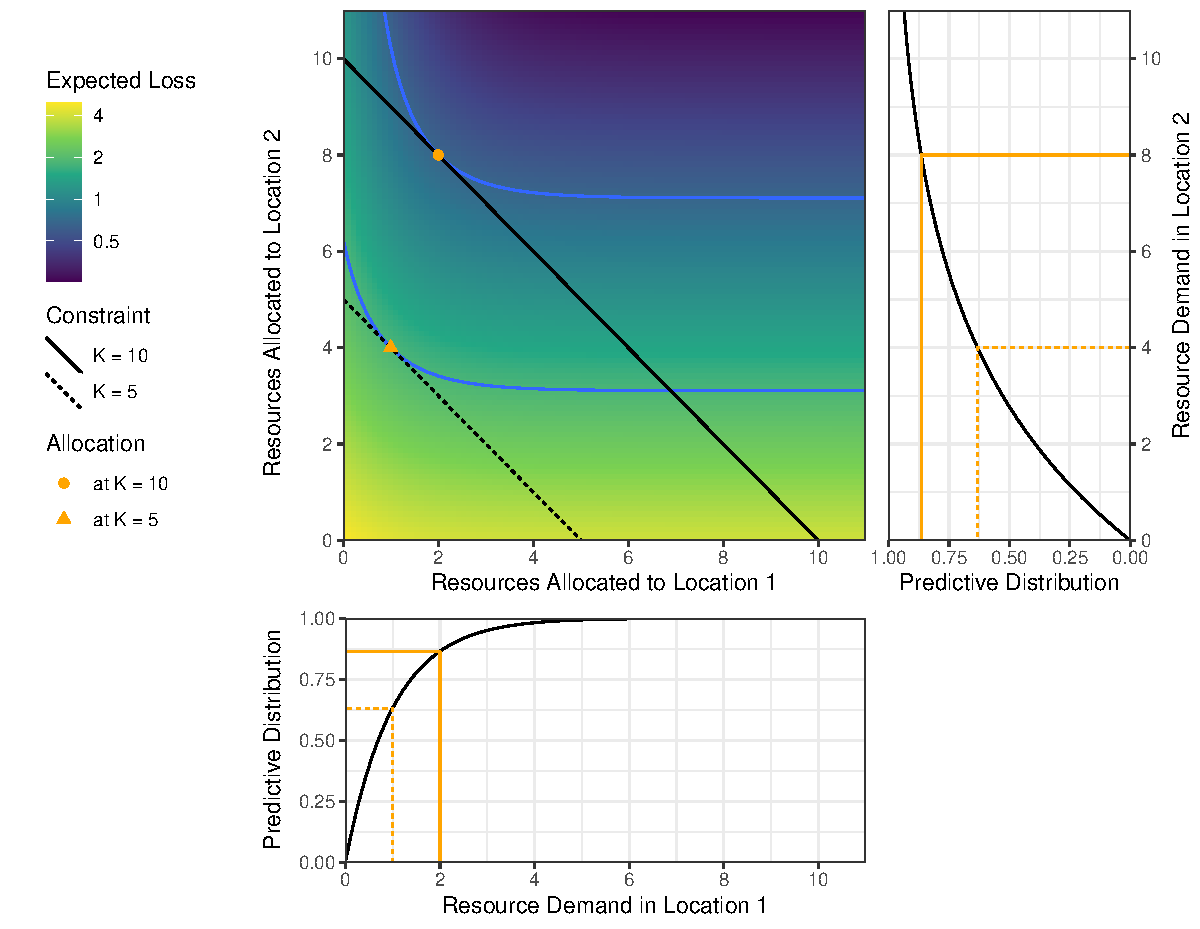
\includegraphics[width=\textwidth]{../figures/exponential_pred_expected_loss.pdf}
    \caption{An illustration of the resource allocation problem in Example 1. There are $N = 2$ locations, with predictive distributions $F_1 = \mathrm{Exp}(1)$ and $F_2 = \mathrm{Exp}(1/4)$. The cumulative distribution functions of these distributions are illustrated in the panels at bottom and right. In the center panel, the background shading corresponds to the expected loss according to these forecasts. Diagonal black lines indicate resource constraints at $K=5$ and $K=10$ units; any point along those lines corresponds to an allocation that meets the resource constraint. For these forecasts, the optimal allocations are $(1, 4)$ for $K=5$ and $(2, 8)$ for $K=10$. These allocations are at the point on the constraint line where the expected loss is smallest, which also corresponds to the point where a level set of the expected loss surface (blue curve) is tangent to the constraint.}
    \label{fig:exp_alloc_example}
\end{figure}

Next suppose that we observe resource needs of 1 and 10 in locations 1 and 2, respectively.
Based on these observed needs, we can measure the quality of the allocation suggested by the forecast by calculating the amount of unmet need that resulted from that allocation over and above what was unavoidable given the resource constraint.
With $K = 5$ units of the resource, the allocation based on the forecast exactly meets the observed need in location 1, but it leaves 6 units of need unmet in location 2.
However, working within the resource constraint, no other allocation could have done better: for example, allocating 0 units of resources to location 1 and 5 to location 2 still results in a total unmet need of 6 across both locations. Therefore, the forecast's allocation score is 0 with $K = 5$.
On the other hand, when $K = 10$, the forecast $F$'s allocation results in $10 - 8 = 2$ units of unmet need in location 2 despite leaving no need unmet in location 1.
In this case, the oracle would be able to prevent all but 1 of the total 11 units of need from going unmet, for example by allocating 1 unit of resources to location 1 and the remaining 9 units of resources to location 2.
The allocation score for the forecast when $K = 10$ would therefore be 1 (= 2 realized $-$ 1 unavoidable) in units of avoidable unmet need.

These scores illustrate a general result: allocation scores for a forecast will tend to be larger when the resource constraint is close to the observed need, because this is when it matters most which locations are allocated more or less resources. If the resource constraint is very small, any allocation of those limited resources will result in a large amount of unmet need. If the resource constraint is very large, it becomes less important which locations receive relatively more or less resources because all locations will receive enough resources to meet their need. In either of these extremes of resource availability, the avoidable unmet need that arises from the allocation suggested by a forecast (i.e., the forecast's allocation score) will tend to be small.

\paragraph{Example 2} Now consider a different forecast that also has exponential distributions for resource need in each location, but that has the scale parameters $\sigma_1 = 2$ and $\sigma_2 = 8$, twice as large as the scale parameters of the forecast in Example 1. Because the optimal allocation is proportional to the scale parameters, this forecast would lead to the same optimal allocations as the forecast in Example 1, and would therefore be assigned the same allocation score.

Note the way in which these forecasts incurred a positive (i.e., non-optimal) allocation score of 1 when $K = 10$. It was not directly due to individual misalignments of the marginal forecasts $F_i$ with the observed needs, but rather because the allocations and observed needs were not proportional as vectors.
Restating: as far as allocation decisions are concerned, with a fixed constraint $K=10$ the fundamental problem with the forecast $F$ in Example 1 is not that it predicts a mean total resource need of $5$ units; it is that the realized need was 10 times as large in location 2 as in location 1, but the forecast only indicated that the resource allocation for location 2 should be 4 times the allocation for location 1.

This illustrates a fundamental property of the allocation score: at its core, it measures whether the forecast accurately captures the relative magnitudes of resource need across different locations, which is precisely the information that is needed to allocate resources to those locations subject to a fixed resource constraint.
On the other hand, the allocation score is not directly sensitive to whether the forecasts in each location correctly capture the magnitude of resource need in each individual location.
%For a given probability level $\tau$, if the quantiles $Q_i(\tau)$ of the marginal forecasts are proportional to the observed needs $y_i$, then the allocation score is zero for the resource constraint level $K = \sum Q_i(\tau)$.
This stands in marked contrast to other common scoring methods for multivariate forecasts that aggregate univariate scores such as log score, CRPS, or WIS for the marginal forecasts where a
poor forecast made for one unit (a location, say) is penalized regardless of alignments in other units. Note that we do not claim that the allocation score is generically preferable to these other scores \textemdash rather, it provides a view of forecast performance that is specifically tuned to the context of decision making about resource allocations.

%It is therefore often straighforward to constuct forecasts $F$ and $\widetilde{F}$ for a given outcome distribution that switch rankings under the allocation and traditional scores by ensuring that the marginal forecasts of $F$ center sharply around allocations that are proportionally similar to the central tendencies of the outcome distribution but are strongly biased.

%While multivariate scoring rules have not seen wide application in infectious disease forecast evaluation, it seems that the allocation score would have a similar relationship with them, since while bias penalties in multi-variate scores can be offset by better forecasting of dependence structure, the proportional biases that allocation scoring are insensitive to are not \emph{per se} tolerated by multivariate scoring rules such as the energy score, variogram score, or Dawid-Sebastiani score.

\subsection{A decision theoretic development of the allocation score}
\label{sec:methods.detailed}

We give a high-level review of a general procedure for developing proper scoring rules that are tailored to specific decision making tasks in section \ref{sec:methods.detailed.decisiontheory}, and then in section \ref{sec:methods.detailed.specific_allocation} we apply that procedure to develop the allocation score based on the task of deciding on how to allocate a fixed supply of resources across multiple locations. In \ref{sec:methods.detailed.integrated_allocation} we consider a small extension where the resource constraint is not known, or it is desired to consider the value of forecasts across a range of decision making scenarios. This gives rise to the \emph{integrated allocation score}.

\subsubsection{The decision theoretic setup for forecast evaluation}
\label{sec:methods.detailed.decisiontheory}

%In this section, we give an overview of the decision theoretic setup for developing proper scoring rules that measure the value of a forecast as an input to decision making. We keep the discussion here at a somewhat informal level; we refer the reader to [some subset of Brehmer and Gneiting; Grünwald and Dawid; Dawid; Granger and Pesaran 2000; Granger and Machina 2006; Ehm et al. 2016] for more technically precise discussion.

In the framework of decision theory, a decision corresponds to the selection of an action $x$ from some set of possible actions $\mathcal{X}$. For example, $x$ may correspond to the level of investment in a measure designed to mitigate severe disease outcomes such as hospital beds, ventilators, medication, or medical staff, with $\mathcal{X}$ being the set of all possible levels of investment that we might select. The quality of a decision to take a particular action $x$ is measured in relation to an outcome $y$ that is unknown at the time the decision is made. For example, $y$ may correspond to the number of individuals who eventually become sick and would benefit from the mitigation measure, and informally, an action $x$ is successful to the extent that it meets the realized need. In the face of uncertainty, a decision maker may use a forecast $F$ of the random variable $Y$ to help inform the selection of the action to take. We measure the value of a forecast as an input to this decision making process by the quality of the decisions that it leads to.

We can formalize the preceding discussion with the following three-step procedure for developing scoring rules for probabilistic forecasts:
\begin{enumerate}
\item Specify a \emph{loss function} $s(x, y)$ that measures the loss associated with taking action $x$ when outcome $y$ eventually occurs.
\item Given a probabilistic forecast $F$, determine the \emph{Bayes act} $x^F$ that minimizes the expected loss under the distribution $F$.
\item The \emph{scoring rule} for $F$ calculates the score as the loss incurred when the Bayes act was used: $S(F, y) = s(x^F, y)$.
\end{enumerate}
%We use the letter $s$ for the loss function to align with the literature on evaluation of forecasts of continuous outcomes, in which context we can often identify the action $x$ with a functional (i.e., a numeric summary such as a mean or a quantile) of the forecast distribution $F$. In this context, $s$ may be used as a \emph{scoring function}. \elr{Consider moving preceding sentences to a footnote or just deleting them?}
This is a general procedure that may be applied in settings where it is possible to specify a quantitative loss function. Subject to certain technical conditions, scoring rules obtained from this procedure are proper. We refer the reader to (cite paper 2 on arxiv) for a more technically precise discussion.

\subsubsection{The allocation score for a fixed resource constraint}
\label{sec:methods.detailed.specific_allocation}

In the decision making setting that we consider, an action $x = (x_1, \ldots, x_N)$ is a vector specifying the amount that is allocated to each of $N$ locations. We require that $0 \leq x$, i.e., that each $x_i$ is non-negative, and that the total allocation across all locations equals the amount of available resources, $K$: $\sum_{i=1}^N x_i = K$. The set $\mathcal{X}$ consists of all possible allocations that satisfy these constraints. The eventually realized resource need in each location is denoted by $y = (y_1, \ldots, y_N)$. These levels of need are not known at the time of decision making, so we define the random vector $Y = (Y_1, \ldots, Y_N)$ where $Y_i$ represents the as-yet-unknown level of resource need in location $i$. Forecasts of need in each location are collected in $F = (F_1, \ldots, F_N)$. We assume that resource need is non-negative and the forecasts reflect that, i.e. the support of each $F_i$ is a subset of $\mathbb{R}^+$. Finally, we assume that each unit of unmet need incurs a loss denoted by $L$, so that if the selected resource level $x_i$ in location $i$ is less than the realized need $y_i$, a loss of $L \cdot (y_i - x_i)$ results. A variety of extensions to this setup are possible; for example, we might account for storage costs for resources that go unused, allow for a different loss per unit of unmet need in each location, or account for resource transportation costs. In this work, we choose to keep the loss function relatively simple to focus on the core ideas.

It is helpful to clearly distinguish between the time $t_d$ when a \emph{d}ecision is made about a public health resource allocation and the time $t_r$ when \emph{r}esource needs that might be addressed by that allocation occur. Our setup assumes that $t_d < t_r$. Additionally, the structure of our loss captures a setting where the resource in question does not impact the amount of demand $y_i$ that will materialize at time $t_r$, but rather it is a resource that satisfies that demand. In the context of infectious disease, this means that we do not consider resources that are intended to reduce the number of people who will become sick at some point in the future, such as a preventative influenza or COVID-19 vaccine. Instead, our set up addresses resources like hospital beds, oxygen supply, ventilators, or rabies vaccines which are intended to meet the medical needs of patients who are already sick. We also note that our problem formulation addresses decision-making that is related to resource needs only at the time $t_r$; we do not explicitly consider sequences of multiple decisions that are made over time or account for the impact of decisions on resource needs at any time other than $t_r$. We outline some opportunities to extend our work to more complex decision making settings in the discussion.

With this problem formulation in place, we can develop a proper scoring rule following the outline in section \ref{sec:methods.detailed.decisiontheory}.

\paragraph{Step 1: specify a loss function.} The loss associated with a particular allocation is calculated by summing contributions from unmet need in each location:
\begin{equation}
s_A(x, y) = \sum_{i=1}^N L \cdot \max(0, y_i - x_i). \label{eqn:loss_fn}
\end{equation}
Here, $\max(0, y_i - x_i)$ is the unmet need in location $i$, which is given by $y_i - x_i$ if the realized need $y_i$ in location $i$ is greater than the amount $x_i$ allocated to that location, or $0$ if the amount $x_i$ allocated to unit $i$ is greater than or equal to the realized need. Also, $L$ is a constant scalar value, the same across all locations, specifying the ``cost'' of one unit of unmet need.

\paragraph{Step 2: Given a probabilistic forecast $F$, identify the Bayes act.} The Bayes act associated with the forecast, $x^{F,K}$, is the allocation that minimizes the expected loss, that is, the solution of the \emph{allocation problem} associated with $K$:
\begin{align}
    \underset{0 \leq x}{\mathrm{minimize}}\,\, \mathbb{E}_{F} [s_A(x, Y)] \text{ subject to }
     \, \sum_{i=1}^N x_i = K, \label{AP}
\end{align}
where $\mathbb{E}_{F} [s_A(x, Y)] = \sum_{i=1}^{N} L \cdot \mathbb{E}_{F_i}[\max(0, Y_i - x_i)]$ sums the expected loss due to unmet need across all locations.

In the supplement we derive a general form of the Bayes act by beginning with the fact that a condition for minimizing expected loss subject to the resource constraint is that there is no way to decrease expected loss further by shifting a small amount of the resource from one location to another.
From this starting point, we can show that the components of the Bayes act are quantiles $x_i^{F,K} = F_i^{-1}(\tau^{F,K})$ at a probability level $\tau^{F,K}$ that depends on the forecast $F$ and the resource constraint $K$, but is shared across all locations. % Compare % In the supplement we derive a general form of the Bayes act by beginning with the fact that a condition for minimizing expected loss under the constraint is that there is no way to decrease expected loss further by shifting a small amount of the resource from one location to another.
% From this, we can show that the components of the Bayes act are quantiles $x_i^{F,K} = F_i^{-1}(\tau^{F,K})$ at a probability level $\tau^{F,K}$ that depends on the forecast $F$ and the resource constraint $K$, but is shared across all locations. % Compare with earlier text: This will lead to the allocations provided by $F$ being quantiles of the marginal distributions $F_i$ for some \emph{single} probability level $\tau$ that is shared in common for all locations.
This probability level is the level at which the resource constraint is satisfied: $\sum_{i=1}^N F_i^{-1}(\tau^{F,K}) = K$.
This tells us that in order to allocate optimally (according to $F$), we must divide resources among the locations so that there is an equal forecasted probability in every location that the allocation is sufficient to meet resource need.
This solution to the allocation problem is well-known in inventory management and is often attributed to \cite{hadleywhitin1963}.

%%%% start of large excision %%%%%

% In the supplement we derive a general form of this solution by beginning with the fact that a condition for minimizing
% expected loss under the constraint is that there is no way to decrease expected loss further by shifting a small amount of the resource from one location to another.
% As a consequence, at $x^{F,K}$, adding resources to any particular location $i$ reduces expected loss at the same rate $\lambda$:
% \begin{align}
% \frac{\partial}{\partial x_i} \mathbb{E}_{F} [s_A(x, Y)] \vert_{x=x^{F,K}} = -\lambda.
% \end{align}
% It turns out that these derivatives can also be expressed in terms of the marginal forecasts $F_i$ as
% \begin{align}
%  \frac{\partial}{\partial x_i} \mathbb{E}_{F} [s_A(x, Y)] = L \cdot (F_i(x_i) - 1)
% \end{align}
% so that
% \begin{align}
% F(x_i^{F,K}) = 1-\lambda/L.
% \end{align}
% This tells us that in order to allocate optimally (according to $F$), we must divide resources among the locations so that there is an equal forecasted probability in every location that the allocation is sufficient to meet resource need.
% It also allows us to write the components $x_i^{F,K}$ of the Bayes act as quantiles
% \begin{align}
% x_i^{F,K} = F_i^{-1}(1 - \lambda/L)
% \end{align}
% which can be substituted into the constraint equation of the allocation problem to get an equation for $\lambda$,
% \begin{align}
% \sum_{i=1}^N F_i^{-1}(1 - \lambda/L) = K.
% \end{align}
% The value of $\lambda$ that solves this equation---which almost always must be approximated with a numerical method---can be substituted back into the quantile formulas
% to arrive at an explicit expression for the Bayes act.
% This partial solution to the allocation problem is well-known in inventory management and is often attributed to \cite{hadleywhitin1963}.
% We note that $\lambda$ and the probability level $1-\lambda/L$ depend on both the constraint level $K$ defining the decision problem and on the forecast $F$. This is quite different from the situation for quantile scores and the WIS, where the probability levels used to calculate scores are fixed.

%%%% end of large excision %%%%%


\paragraph{Step 3: Define the scoring rule.} We can now use the Bayes act to define a proper scoring rule for the probabilistic forecast $F$.
Consider first the ``raw'' score defined as
\begin{align}
S_A^{\text{raw}}(F, y; K) = s_A(x^{F,K}, y) = \sum_{i=1}^N L \cdot \max(0, y_i - x_i^{F,K}).
\end{align}
This measures the total unmet need across all locations that results from using the Bayes allocation associated with the forecast $F$ when the actual level of need in each location is observed to be $y_i$.

To make this a more easily interpreted measure of forecast performance, we will adjust the raw score by subtracting the minimum loss $l_{\text{oracle}}(y;K)$ achievable by an \emph{oracle} allocator which has precise foreknowledge of the outcomes $y_i$.
This minimum loss is given by $l_{\text{oracle}}(y;K) = L \cdot \max(0, \sum_{i=1}^{N}y_i - K)$: if there are enough resources to meet the total resource need ($\sum_{i=1}^{N}y_i \leq K$), the oracle can achieve a loss of 0, but if the resource constraint is less than the total needed resources ($\sum_{i=1}^{N}y_i > K$), it is not possible to do better than a loss of $L \cdot (\sum_{i=1}^{N}y_i - K)$.

Our scoring rule is then given by
\begin{align}
S_A(F, y; K) &= S_A^{\text{raw}}(F, y; K) - l_{\text{oracle}}(y;K) \\
& =
\begin{cases}
\sum_{i=1}^n L  \cdot  \max(0, y_i - x_i^{F,K}), &  \sum_{i=1}^{N}y_i \leq K \\
L \cdot K - L \cdot \sum_{i=1}^{N} \min(x_i^{F,K}, y_i), &  \sum_{i=1}^{N}y_i > K.
\end{cases}
\end{align}
In the first case, the oracle incurs no loss so that the raw and adjusted scores coincide. The second case can be read as taking the $K$ resource units perfectly allocated by the oracle as a base penalty on
the imperfect forecast $F$ and then, for each location $i$, reducing this penalty by however much of the need $y_i$
is met with the Bayes act component $x_i^{F,K}$.
The oracle adjustment aligns with the idea that \emph{opportunity loss} (often known as \emph{regret} or (negative) \emph{relative utility}) is often a more important quantity than absolute loss \elr{needs citation}.

\subsubsection{Integrating the allocation score across resource constraint levels}
\label{sec:methods.detailed.integrated_allocation}

The allocation score $S_A$ that we developed in the previous section measures the skill of the forecast distributions $F$ based on a single probability level $\tau^{F,K}$. This is appropriate if the resource constraint $K$ is a known constant. However, if $K$ is not precisely known at the time of decision making or there is interest in measuring the value of forecasts across a range of decision making scenarios with different resource constraints, we can use an \emph{integrated allocation score} (IAS) that integrates the allocation score across values of $K$, weighting by a distribution $p$:
$$S_{IAS}(F, y) = \int S_A(F,y; K) p(K) \, dK$$
We note that the device of considering a range of hypothetical decision makers or decision making problems with different problem parameters has been employed in the past \cite[e.g.,][]{murphy1993whatisagoodforecast}.

\subsection{Generalizations and Connections to Other Scores}
\label{sec:methods.related}

We begin this section by briefly sketching how the weighted interval score (WIS), a commonly used proper scoring rule for probabilistic forecasts during the COVID-19 pandemic, can be derived using the decision theoretic approach above. Then, we discuss similarities and differences between WIS and the allocation score, and other scores in general.

\subsubsection{The quantile loss and weighted interval score (WIS)}
\label{sec:methods.wis}

The weighted interval score (WIS) was proposed in 2020 as a way to score forecasts that were being made in the early stages of the COVID-19 pandemic \citep{bracher2021evaluating}; equivalent scores had also been used in previous forecast evaluation efforts \cite[e.g.,][]{hong2016probabilisticEnergyForecasting}.
The WIS is a proper scoring rule for forecasts that use a set of quantiles to represent a probabilistic forecast distribution.
%% optional detail
Many early COVID-19 modeling efforts, including the US COVID-19 Forecast Hub and other collaborative forecasting projects, adopted a quantile forecast format as a matter of convenience (e.g., this format does not require the forecaster to pre-specify an upper bound for disease counts as would be required to collect forecasts in the format of bin probabilities) \citep{cramer_united_2022}.
%%
While pointing a reader interested in more mathematical detail to \cite{bracher2021evaluating}, we note simply that the WIS is a weighted sum of interval scores at different probability levels (e.g., 50\% prediction intervals, 80\% PIs, 95\% PIs, etc...).
Larger interval scores indicate less skillful forecasts.
An interval score consists of (a) the width of the interval, with larger intervals receiving higher scores, and (b) a penalty if the interval does not cover the eventual observation, which increases the further away the interval is from the observed value.
Equivalently, the WIS can also be characterized as a weighted sum of quantile scores for each individual predictive quantile.
The quantile score for a particular quantile level assigns an asymmetric penalty to predictions that are too high or too low, with the relative sizes of the penalties set so that in expectation the score is minimized by the given quantile of the distribution.
The most commonly used version of WIS is one that uses an equal weighting of all quantile levels, in which case WIS approximates the continuous ranked probability score (CRPS), a commonly used score for probabilistic forecasts.
\apg{Maybe a rewording and/or a supplement reference here to mention that any WIS approximates the a corresponding weighted CRPS, and that WIS actually is the wCRPS for a discrete measure/weighting.}
\emph{It is important to note that this weighting was proposed because the resulting score approximates the CRPS, and not because it aligned with any particular public health decision-making rationale.}

That said, the quantile score and WIS can be derived using the same decision theoretic procedure that we outlined in section \ref{sec:methods.detailed}.
In fields such as meteorology and supply chain management, a great deal of attention has been given to the problem where a decision must be made about the quantity of a resource to purchase for a single location in the face of a fixed cost $C$ for each unit of the resource and a loss $L$ that will be incurred for each unit of unmet need.
This leads to the quantile score for the probability level $\tau = 1 - C/L$.
From this point, the WIS or CRPS can be obtained by averaging across a range of decision making settings with different cost and loss parameters, using a similar motivation that we used to obtain the IAS from the AS in section \ref{sec:methods.detailed.integrated_allocation}.
\apg{Refs to supp for quantile score derivation and detail about averaging.}
%\ngr{I might suggest adding a detailed Step 1/2/3 as an appendix and referencing it here. But I think that adding that full detail here might be too much.}
%\ngr{can we make more explicit the link here to the section above? I'm not confident in my ability to describe with technical accuracy the link between quantile/pinball loss and CRPS, but I think this is a good opportunity to do so briefly.}

\subsubsection{Connections between scores}
\label{sec:methods.generalization}

We have described in previous sections how both the allocation score and the weighted interval score (WIS) arise from a single standard procedure for developing proper scoring rules.
The allocation score arises when the decision relates to how a fixed quantity of resources should be allocated to multiple locations.
The WIS and CRPS arise when the decision relates to how much of a resource to order in the context of the cost of the resource and wanting to minimize unmet need in one or more locations.
In both settings, the optimal solution sets the resource level in each location to a quantile of the respective forecast distributions.

These decision making problems differ according to the challenge faced by the decision maker: a fixed constraint on the available resources for the allocation problem, or a cost per unit of resources in the resource purchasing problem. In fact, it is possible to combine these into a more general problem where the decision maker must decide on both the total level of resources to purchase and an allocation of those resources across multiple locations, subject to a cost per unit of resources and a constraint on the total quantity of resources that can be purchased. The quantile loss and the allocation score presented in this work are both special cases of the score that emerges from that more general decision making problem that integrates across resource cost and constraint parameters together. We pursue this direction further in other work that is in progress.

\section{Evaluating forecasts of COVID hospitalizations using the allocation score}
\label{sec:application}

We illustrate with an application to hospital admissions in the U.S., considering the problem of allocation of a limited supply of medical resources to states.

\begin{figure}
    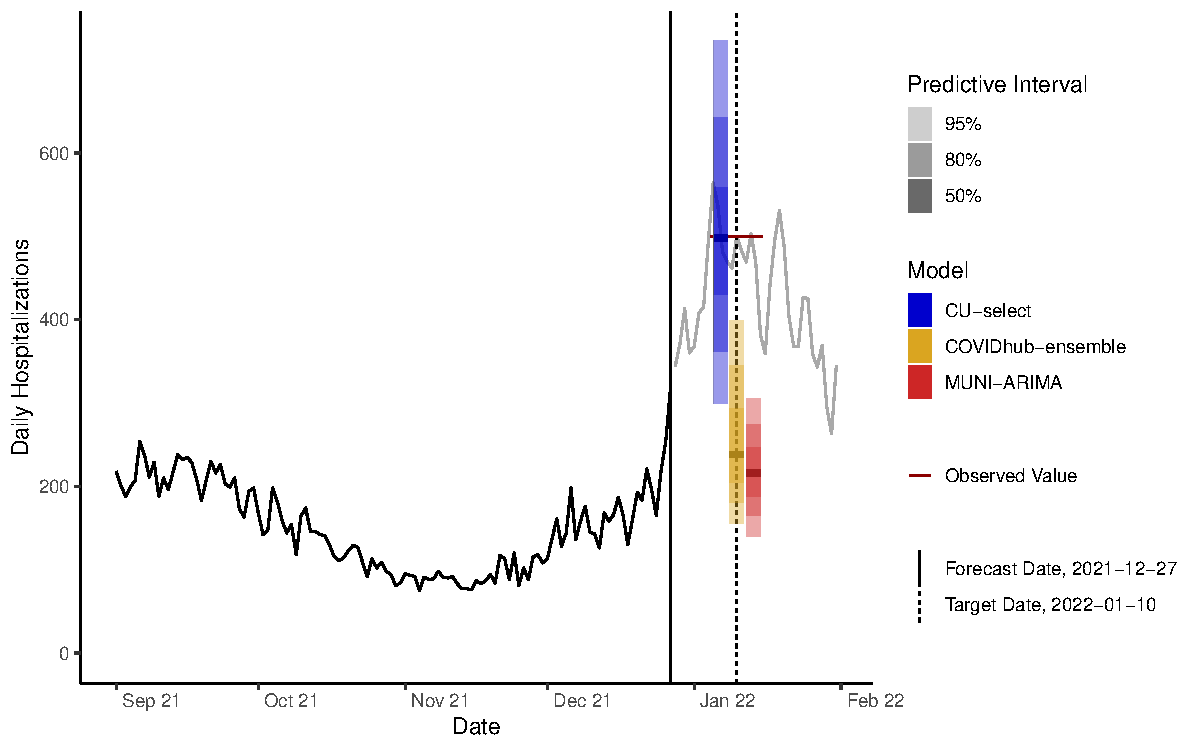
\includegraphics[width=\textwidth]{../figures/allocation-forecasts-v2.pdf}
    \caption{Hospitalization data and example forecasts for Virginia, US. New daily hospital admissions are shown by the line of data. The dark line indicates data up to the time the forecast was made on December 27, 2021; the grey line indicates data available in retrospect. The set of colored bars represent forecasts made for 14 days into the future, with a target date of January 10, 2022 (dashed vertical line). The horizontal dashed line indicates the level of the observed value on this day. Note that all three forecasts correspond to forecasts for the same day, but they are spread out for better visibility. }
    \label{fig:sample-forecasts}
\end{figure}


\subsection{Data}



\subsubsection{Hospitalization data}
Starting in the summer of 2020, the US Health and Human Services began reporting counts of daily new admissions to hospitals for individuals with COVID-19.\citep{healthdatagov_covid-19_nodate}
These data served as the source of ``ground truth'' data for the US COVID-19 Forecast Hub which, starting in December 2020, collected short-term forecasts of new hospital admissions at the daily scale.
These daily counts were available for the US as a whole, and all states and several additional jurisdictions such as Puerto Rico and Washington DC.
The data were updated daily and were available for download by the public through the HHS HealthData.gov website.
For this analysis, we downloaded the hospitalizations data through the covidHubUtils R package, which connects users to the most recent version of the data.\cite{wang-covidhubutils}
The hospitalization data were downloaded for analysis on 2023-10-29.

\subsubsection{Forecast data}
The US COVID-19 Forecast Hub, a consortium funded by the US CDC and led by a research group at UMass-Amherst, collected short-term forecasts of hospitalizations starting in December 2020.\citep{cramer_united_2022}
Any team that with appropriately formatted forecasts could submit them to the Forecast Hub data repository on GitHub.(cite repo site)
Forecasts were time-stamped by GitHub upon submission and passed validation checks that ensured correct formatting and that the forecasts were being submitted only for dates in the future, not for data that had already been observed.

Forecast submission followed a weekly cycle and culminated in the creation of an ensemble forecast.
Forecasts could be submitted on any day during the week.
However once a week on Mondays, the Forecast Hub would collect the most recent forecasts submitted by all teams that met certain inclusion criteria and create an ensemble forecast using quantile averaging.\citep{ray_comparing_2023}
An ensemble that treated all models equally was created (COVIDhub-ensemble) as was a model that created weights of submitted models based on performance in the past 12 weeks (COVIDhub-trained\_ensemble).
One other model that combined multiple forecasts from different teams but used a different ensembling algorithm, a linear pooling method with tail extrapolation, was also included in our analyses (JHUAPL-SLPHospEns).
Several other models have ``ensemble'' in their name, but this refers to combinations of different variations of models that the specific team created, not to a multi-model ensemble combining different submitted forecasts to the Forecast Hub.

All forecasts, including the ensemble, were submitted as probabilistic predictions about the number of new hospital admissions on a particular day in the future, in a specific jurisdiction of the US (national level, state, or territory).
Probability distributions were specified, per the requirements established by the Forecast Hub, as a set of 23 quantiles for each individual prediction.
The submitted quantiles included a median (treated as a ``point'' prediction) and defined 11 central prediction intervals, from a 99\% to a 10\% prediction interval.

The analysis in this work focuses on forecasts made before and during the first wave of the Omicron SARS-CoV-2 variant in the US.
As such, we downloaded forecasts for the 15 weeks starting with Monday 2021-11-22 through Monday 2022-02-28.
Forecast data were downloaded on for analysis on 2023-10-06.


We established a set of inclusion criteria to determine which forecasts and models to include in our analysis.
Models were eligible to be included in the analysis if they were considered a ``primary'' model from a team. (If a team submitted multiple versions of similar models, they were required to designate one as ``primary''.)
For a model to have a complete, eligible submission in a given week, it had to have a 14 day-ahead forecast for all 50 states plus Washington DC.
Models had to have a complete forecast for at least 4 of the 15 weeks in the analysis to be considered eligible for inclusion.

\subsection{Evaluation metrics}

This manuscript focuses on two proper forecast scores, the allocation score and the weighted interval score (WIS), both defined above.

\subsubsection{Allocation Score}

For this analysis, we fixed a resource constraint $K$ to be 15,000, based roughly on a reported number of ventilators available for reallocation in the US.\citep{ajao_assessing_2015}
For each week, we computed a the allocation score for each 14 day-ahead forecast based on $K=15,000$.

We also computed a standardized rank for the allocation score for each model $m$ and week $w$.
First, we computed the number of models that forecasted that week ($n_w$) and the rank of model $m$ among the $n_w$ models ($r_{m,w}^{AS}$).
The model with the best allocation score received a rank of 1 and the worst received a rank of $n_w$.
In the case of a tie between one or more models, all models received the better rank.
We then rescaled these rankings to compute the allocation score standardized rank ($sr_{m,w}^AS$) between 0 and 1, where 0 corresponds to the worst rank and 1 to the best.


\begin{equation}
sr_{m,w}^{AS} = 1 - \frac{r^{AS}_{m,w}-1}{n_w-1}
\end{equation}

\subsubsection{Weighted Interval Score (WIS)}

The Weighted Interval Score (WIS), as described in earlier sections, measures the alignment of a single probabilistic forecast ($F$) with an observation ($y$).
We computed the mean WIS across all $L$ locations for each model and each forecasted week as
\begin{equation}
MWIS_{m,w} = \frac{1}{L}\sum_{l=1}^L WIS(F_{l,m,w},y)
\end{equation}
where $F_{l,m,w}$ is the probabilistic forecast from model $m$ for location $l$ and week $w$.
Using the same procedure as for allocation scores described above, we computed standardized ranks for MWIS ($sr_{m,w}^{MWIS}$).

\subsection{Data and code availability}

\subsection{Application results}




\subsubsection{Forecast scores showed differences over time}



\begin{knitrout}
\definecolor{shadecolor}{rgb}{0.969, 0.969, 0.969}\color{fgcolor}\begin{figure}
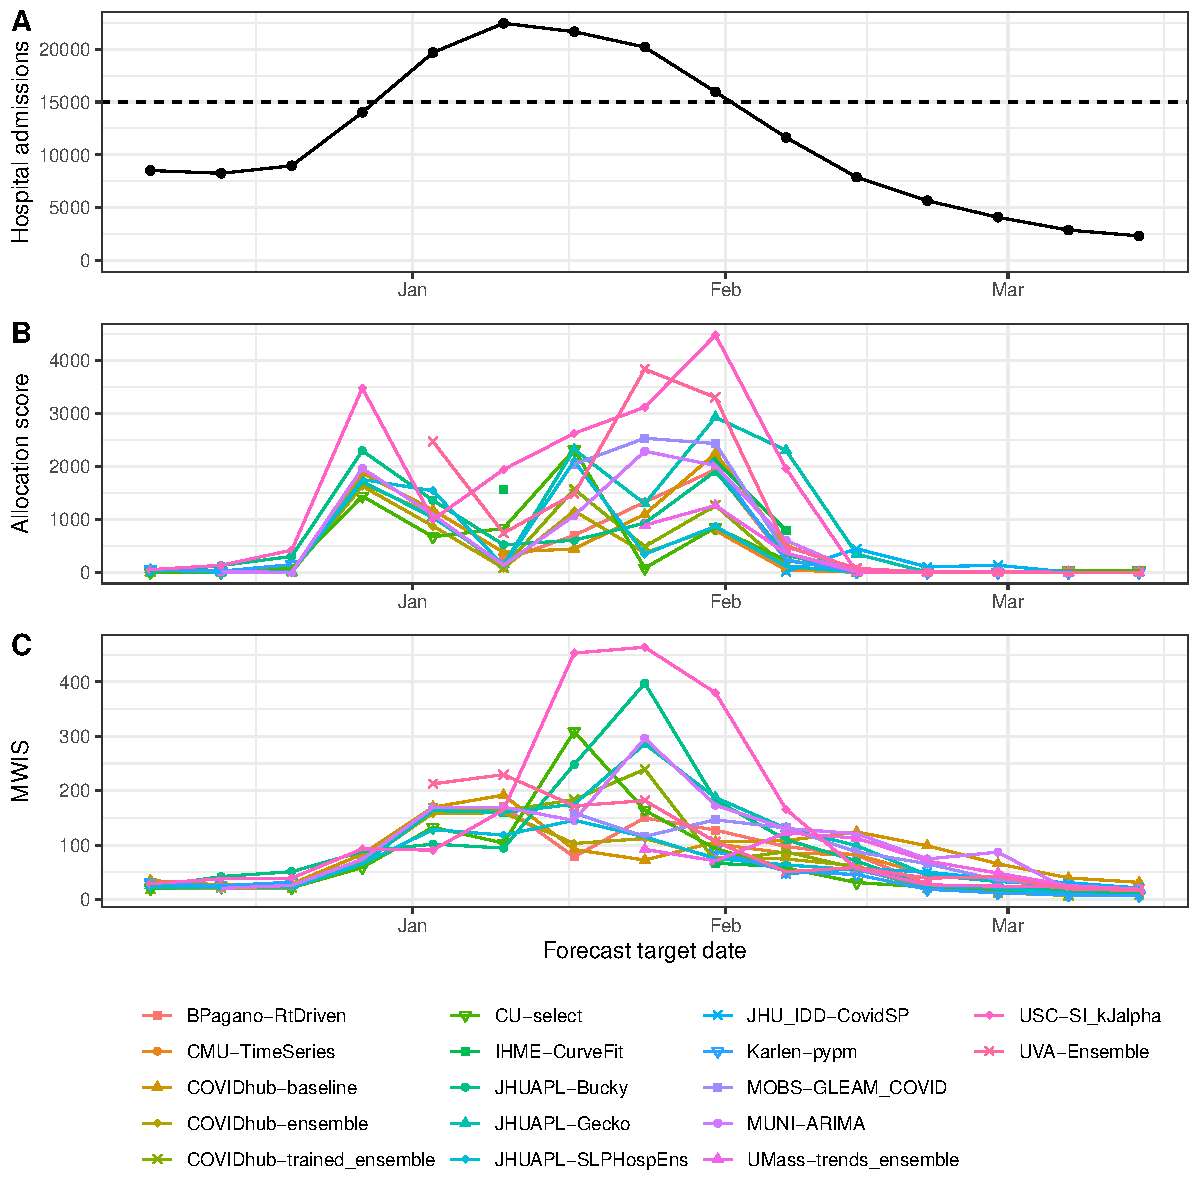
\includegraphics[width=\maxwidth]{figure/metrics-over-time-1} \caption[Hospital admissions and evaluation metrics over time]{Hospital admissions and evaluation metrics over time. Panel A shows the number of hospital admissions in the US as a whole due to COVID-19 on a sequence of 15 Mondays from December 2021 through March 2022. These are the days for which forecasts were made and evaluated. A horizontal dashed line at 15,000 shows the assumed resource constraint $K$. Panel B shows allocation scores for each model's 14-day ahead forecast, across all US states. The x-axis corresponds to the date for which the prediction was made. Allocation scores typically are high when the observed value is near to the constraint, which occurs during the last Monday in December (on the way up) and the last Monday in January (on the way down). Panel C shows the MWIS metric across weeks, averaged across all states. Similarly to panel B, the x-axis corresponds to the date for which the prediction was made. MWIS values tend to scale with the observed and predicted values, and the peak MWIS values happen around and just after the pean of the Omicron wave.}\label{fig:metrics-over-time}
\end{figure}

\end{knitrout}

Allocation scores varied substantially by date and by model (Figure \ref{fig:metrics-over-time}).
For predictions made for the first three Mondays in December 2021 and the last three Mondays in February 2022 all models had allocation scores under 500 (and the mean across all models was less than 100), indicating that the unnecessary unmet need was fairly low relative to the total number of hospital admissions on those days.
The allocation scores are on the whole highest when the observed number of new hospital admissions is closest to the resource threshold of 15,000, as this is the time when any mistakes in allocation are costly in terms of wasting resources in one location that could have been used in another.
Predictions made during the peak week and just after showed the highest variation in allocation scores, with some models having allocation scores under 1000 and others having values over 3500.



Overall, across the first 11 weeks evaluated (we excluded the last four since nearly all the models achieved an allocation score of zero), the \texttt{COVIDhub-baseline} model, which predicts a flat line from the most recent observation with uncertainty bounds based on a random walk, had the highest rank for allocation score in four weeks, more than any other model except the \texttt{COVIDhub-ensemble} which also had four.




Mean weighted interval scores (MWIS) also varied by date and model, and more clearly were dependent on the scale of the observed data.
MWIS values were low (all models under 100) for all Mondays in December 2021 and the final four Mondays evaluated.
Across all models both the average and median MWIS value for every Monday in January was above 100, with the largest errors occurring one and two weeks after the peak was observed.



\subsubsection{Model rankings for different scores did not reliably correlate}

\begin{knitrout}
\definecolor{shadecolor}{rgb}{0.969, 0.969, 0.969}\color{fgcolor}\begin{figure}
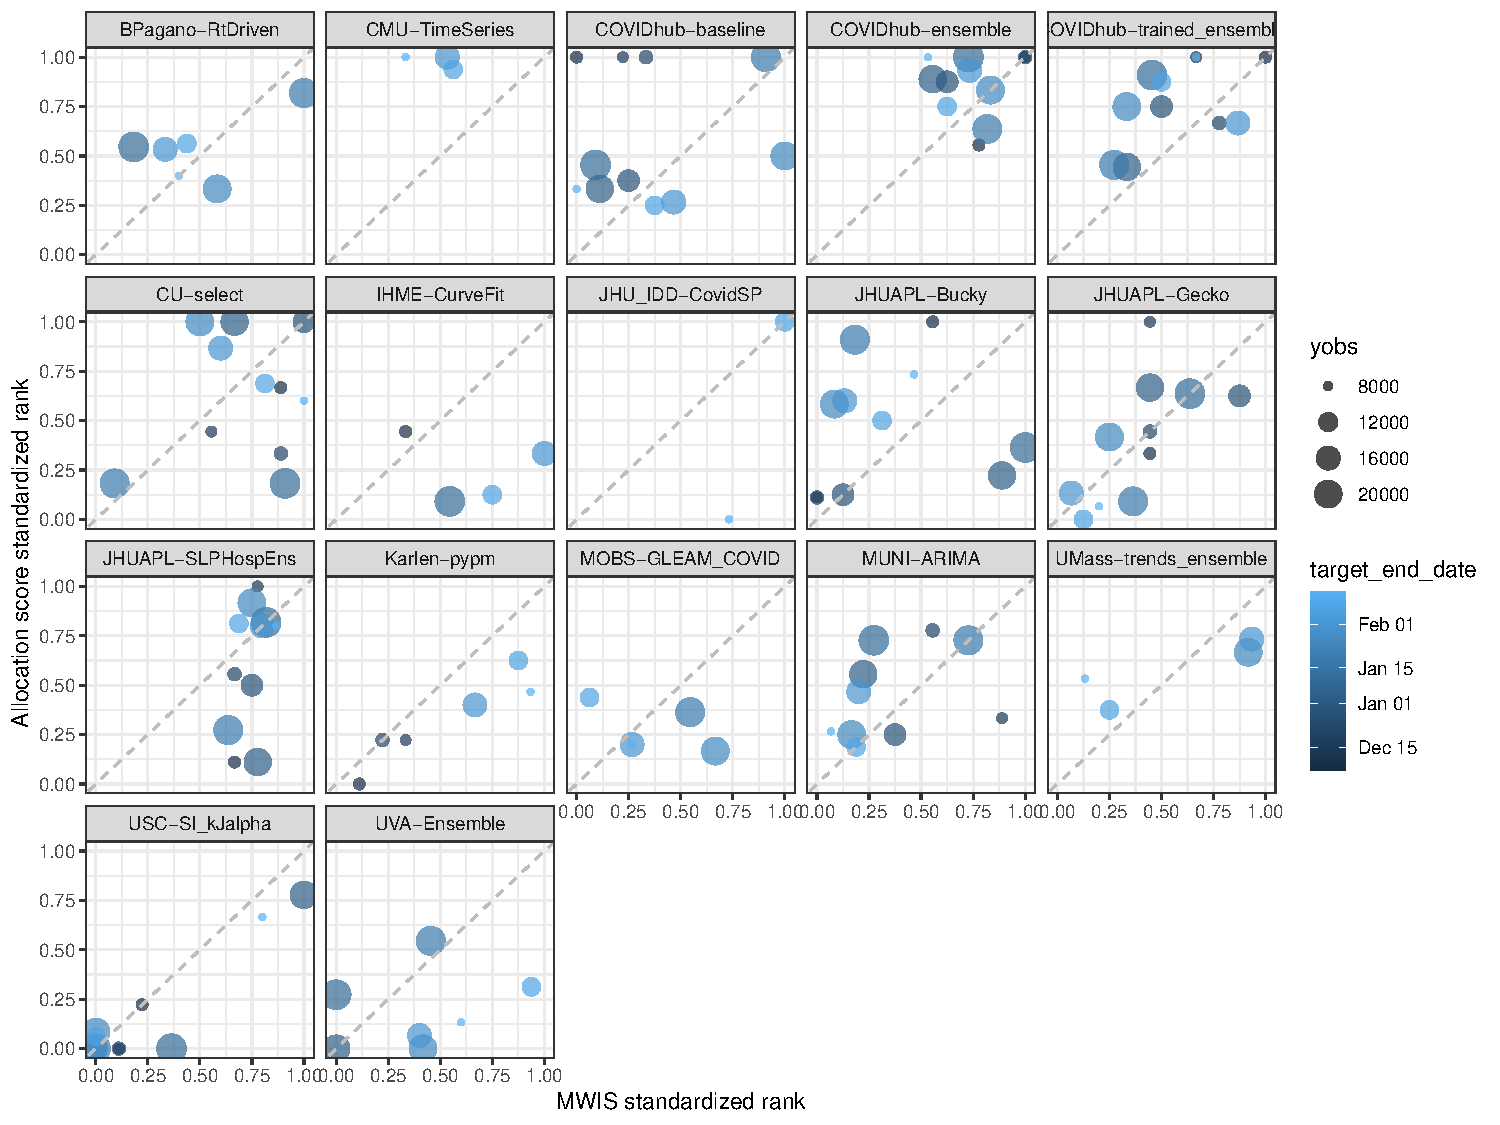
\includegraphics[width=\maxwidth]{figure/metrics-correlation-1} \caption[Association of standardized ranks for MWIS and allocation score by model and week]{Association of standardized ranks for MWIS and allocation score by model and week. Each facet of the plot corresponds to one model. Within each facet, each point corresponds to a week. The x- and y-values correspond to the MWIS standardized rank and the allocation score standardized rank for that week. Points corresponding to earlier dates have darker shading. The size of the point corresponds to the observed value on the date for which the prediction was made. Models show different degrees of association between the two metrics.}\label{fig:metrics-correlation}
\end{figure}

\end{knitrout}

Models showed differing levels of correlation between their allocation scores and MWIS values (Figure \ref{fig:metrics-correlation}).
Here are some examples of the different model-specific patterns observed:
\begin{itemize}
\item Several models showed a positive association between allocation score and MWIS ranks (e.g., \texttt{Karlen-pypm} and \texttt{USC-SI\_kJalpha}).
\item Several models had consistently strong MWIS ranks but also had highly variable allocation score ranks with no clear association between the two (e.g., \texttt{JHUAPL-SLPHospEns} and \texttt{CU-select})
\item One model performed consistently well for both metrics with no clear association (\texttt{COVIDhub-ensemble})
\item One model performed consistently well for allocation score but had only middlings ranks for MWIS (\texttt{CMU-TimeSeries})
\end{itemize}




\subsubsection{Integrated allocation score across values of K}

Using the integrated allocation score summarizes allocation scores across a range of possible values of the constraint ($K$) (Section \ref{sec:methods.detailed.integrated_allocation}).
This could be useful in situations where the actual constraint may not be known, or could only be specified as a probability distribution.

 - something here from Ben's analysis?


\ngr{include figure here that shows relative rankings of locations?}

\section{Discussion}
\label{sec:discussion}

All proper scoring rules for probabilistic forecasts have an explicit link to a loss function, thereby placing numerical value on different kinds of errors in specifying forecasts.
In epidemiological forecasting, well-known proper scoring rules such as the log score or variations on the continuous rank probability score (such as the weighted interval score, or WIS) have been frequently utilized to evaluate probabilistic forecasts.
Often, these scores are used to rank models according to accuracy with that particular score, but without reference to the underlying decision-making process for which that score was designed.
With careful thought and collaboration between modelers and public health officials, we argue that scores that are more aligned with public health decisions could be developed to inform specific problems.
We have demonstrated that forecast evaluation methods that are tied to a specific decision making context can yield model rankings that are substantively different from standard measures of forecast skill.

We often conceive of infectious disease forecasts as being useful for decision making purposes, but it is rare for forecast evaluation to be tied directly to the value of the forecasts for informing those decisions. This work seeks to address that gap.
However, we do note that the decision-making context presented in this work, while motivated by examples from real-world public health resource allocation problems, has not used to inform an actual real-time decision-making process.

Resource allocation decisions are a realistic example of the kinds of decisions that could motivate more targeted forecasting exercises.
One real-world example is allocation of ventilators during a respiratory viral pandemic.
This was the motivating example for the examples presented in the work above.
However, other examples where allocation is a central concern exist as well, such as the allocation of a limited stockpile of vaccinations\citep{persad_fair_2023} or diagnostic tests\citep{du_optimal_2022}.

In practice, there are many potential users of forecasts with many different decision making problems.
Not all can be easily quantified.
Those that can be easily quantified may differ enough that it seems likely that no single score would be appropriate for all users.
In an ideal setting, a forecasting tool could be developed through close collaboration between modelers and public health officials.
However, this setting may only be possible in settings with enough resources to support both an analytics and public heatlh team.
Increasingly, collaborative modeling hubs are being used to generate ``one-size-fits-all'' forecasts for many locations at once.
In these settings, where tailored models are not available, it still could be possible to evaluate contributed models against a set of multiple scores.
% NGR: leaving this out for now as it feels like too much detail?
% This may be tricky to operationalize in the setting of a general forecast hub. It matters how you elicit and represent probabilistic forecasts (quantiles? samples? cdfs?).


In our specific application, we made several key observations that we believe should inform future work in this area.
First, it is clear that different metrics (in our case allocation score and mean weighted interval score) captured different aspects of forecast performance.
The MWIS was strongly dependent on the scale of the forecasted quantity (e.g., when hospitalizations were high, so was WIS).
The allocation score was not as scale-dependent, as the highest/worst allocation scores were observed when the number of hospitalizations was closest to the allocation constraint.
We also note that contributed models found it hard to have a better allocation score than a na\"ive baseline model that just predicted a flat line from the last previous observation with wide uncertainty.
This suggests suggests that contributed models (other than the ensemble, which combined forecasts from all contributed models) were not consistently adding value over just extrapolating from the current levels.


There are several important limitations to the current work.
The allocation score we developed here does not directly account for important considerations such as fairness or equity of allocations.
Nor does the proposed framework attempt to capture the broader context of decision making. For example, in practice it may be possible to increase the resource constraint $K$ by shifting funding from other disease mitigation measures.
We also note that in some settings, a ``successful'' epidemiological forecast may lead to policy decisions that change the distribution of the predicted outcome $Y$. Our framework cannot be used to evaluate a forecast at a horizon that may have been impacted by such a decision.

We see this work as an initial overture for what we hope will grow to be a large, collaborative body of work in more closely coupling applied epidemiological forecasting with public health decision-making.
We note that a few papers have begun exploring similar linkages as described in the literature review \textendash but we see much room for additional work in this area.
In some situations, individual or ensemble models could be developed to optimize scores that are attunend to a particular decision making setting.
This area is also largely unexplored in the realm of public health to date, with some initial methodological development in econometrics \citep{loaiza-maya_focused_2021}.

In conclusion, we argue that the way modelers and policymakers view and evaluate forecasts should change depending on the specific decision-making context.
Using standard forecast evaluation metrics can mask the utility of certain forecasts, or lead to forecasts being used to inform a particular decision that are not optimal for that particular set of values that are important for that context.
Further collaborative work is needed to assess the value and relevance of the initial findings presented here, including real-time pilot studies or simulation exercises that could be used to inform further development of new or alternative scoring metrics.


\bibliography{allocation}

\end{document}
